\documentclass[journal]{IEEEtran}

\usepackage{color}
\usepackage{float}
\usepackage{amssymb}
\usepackage{cite}
\usepackage{amsmath}
\usepackage{amsthm}
\newtheorem{Statement}{Statement}
\usepackage{enumerate}
\usepackage{algorithm}
\usepackage{algpseudocode}
\usepackage{graphicx}
\usepackage{epstopdf}
\epstopdfsetup{outdir=./}
\graphicspath{{../Images/}{../}}
\usepackage{booktabs}
\usepackage{multirow}
\usepackage{bm}
\usepackage{url}
\usepackage{tabularx}
\usepackage{placeins}
\newcommand{\revision}[1]{\textcolor{blue}{#1}}
\setlength{\textfloatsep}{5pt plus 1pt minus 1pt}
\setlength{\floatsep}{5pt plus 1pt minus 1pt}
\setlength{\intextsep}{5pt plus 1pt minus 1pt}
\setlength{\abovedisplayskip}{4pt plus 1pt minus 1pt}
\setlength{\belowdisplayskip}{4pt plus 1pt minus 1pt}
\setcounter{topnumber}{5}
\setcounter{bottomnumber}{5}
\setcounter{totalnumber}{10}
\renewcommand{\topfraction}{0.95}
\renewcommand{\bottomfraction}{0.90}
\renewcommand{\textfraction}{0.05}
\renewcommand{\floatpagefraction}{0.85}
\renewcommand{\dbltopfraction}{0.95}
\renewcommand{\dblfloatpagefraction}{0.85}

% Correct bad hyphenation here
\hyphenation{op-tical net-works semi-conduc-tor}

\begin{document}

\title{MAML-Select: An Online Adaptive Client Selection Method for Federated Learning via Meta-Learning}

%\author{Aakash Sharma, Advait Pathak, Ricktho Sarkar, Om Jee Pandey, \textit{Senior Member, IEEE}
%\thanks{A. Sharma, A. Pathak, and R. Sarkar are undergraduate researchers at IIT BHU Varanasi, Varanasi 221005, India.}
%\thanks{O. J. Pandey is with the Department of Electronics Engineering, IIT BHU Varanasi, Varanasi 221005, India (e-mail: omjee.ece@iitbhu.ac.in).}}

\maketitle

% =====================================================================
% ABSTRACT
% =====================================================================
\begin{abstract}
Federated Learning (FL) enables collaborative model training across edge devices\revision{ but remains constrained by non-IID data and heterogeneous client resources. Client usefulness also changes during training, so a fixed selection rule can become stale. We propose \textbf{MAML-Select}, an online adaptive client-selection method that meta-learns a lightweight ranking policy and adapts it from recent round feedback before selecting the next cohort. The policy is a $6$-$64$-$64$-$1$ MLP with 4,673 trainable parameters and uses observed local loss reduction and latency-aware cost feedback. Across Fashion-MNIST, CIFAR-10, and CIFAR-100 with 100 clients, $K=10$, Dirichlet $\alpha=0.5$, and three random seeds, MAML-Select achieves accuracy competitive with FedAvg and FedGCS while reducing cumulative training TFLOPs by $12.8\%$, $21.5\%$, and $1.7\%$ relative to FedAvg. The corresponding modelled energy/carbon reductions are $16.4\%$, $24.7\%$, and $4.7\%$. The largest accuracy trade-off occurs on CIFAR-10 ($-3.8$ percentage points), where the resource reduction is also strongest. Sensitivity and ablation studies show that the trade-off parameter and six state features behave stably.}
\end{abstract}
\renewcommand\IEEEkeywordsname{Impact Statement}
\begin{IEEEkeywords}
This work addresses the challenge of deploying FL in heterogeneous \revision{environments, including the} Internet of Vehicles (IoV), mobile healthcare, smart-city sensing, and industrial \revision{Internet of Things}. \revision{MAML-Select is intended for settings where participation decisions must balance model quality with limited client compute, latency, and energy budgets. Its impact is therefore efficiency-oriented: it provides a reproducible way to trade small accuracy changes for lower simulated computation and lower model-based energy/carbon cost. These estimates are tied to the stated client-tier power and grid-intensity assumptions, and future work will validate the method on physical heterogeneous devices with hardware-level energy measurement.}


%This enables more scalable and energy-efficient privacy-preserving AI on resource-constrained edge devices.
\end{IEEEkeywords}
\renewcommand\IEEEkeywordsname{Index Terms}
\begin{IEEEkeywords}
Federated learning, client selection, meta-learning, and computational efficiency.
\end{IEEEkeywords}
% =====================================================================
% I. INTRODUCTION
% =====================================================================
\section{Introduction}

\IEEEPARstart{F}{ederated} Learning (FL) has emerged as \revision{an important} framework for privacy-preserving distributed intelligence~\cite{mcmahan2017communication}. \revision{Clients train models locally and share only model updates with a central server. FL clients vary in hardware capabilities, network conditions, and local data distributions. This heterogeneity creates two coupled challenges. Statistical heterogeneity causes client drift under non-IID data, while system heterogeneity allows stragglers to dictate round latency in synchronous protocols}~\cite{karimireddy2020scaffold,mai2024study,tapwal2026stragglers,forootani2026asynchronous}. \revision{Recent work also revisits the definition of non-IID data for computer-vision tasks}~\cite{borazjani2026redefining}. Despite these advances, the fundamental problem of \textit{whom to select} for each training round remains an open challenge.

Client selection, the process of choosing a subset $\revision{\mathcal{S}_t} \subset \{1, \ldots, N\}$ each round, is thus a focal point of FL research. \revision{A client that is useful early in training may become redundant later. Conversely, a previously overlooked client may become important.} System-aware methods maximize feasible participation under latency and resource constraints\revision{. However, they may bias the model against} slow yet data-rich clients~\cite{nishio2019client,chai2020tifl}. Utility-aware methods prioritize statistical information gain\revision{, but some incur high latency or expensive server-side modelling}~\cite{lai2021oort,tang2022fedcor,xu2024federated,yan2023criticalfl,ning2024fedgcs}. Learning-based selectors use interaction histories, contextual features, or reinforcement signals to adapt participation decisions~\cite{wang2020optimizing,pan2024contextual,kazemi2026robust}. \revision{These approaches address important aspects of client selection. However, an efficient round-by-round mechanism for adapting the ranking policy to evolving client utility remains underexplored.}

\revision{In this paper, we propose MAML-Select, a client-selection framework based on a MAML-style fast adaptation step}~\cite{finn2017model}. \revision{MAML-Select learns an initialization for a policy network. Recent feedback is used to rapidly adapt the policy before the next client-ranking decision. Unlike RL-based and contextual-bandit selectors, our focus is rapid gradient-based adaptation of the ranking policy across FL rounds. This is also distinct from FL personalization methods}~\cite{fallah2020personalized}. \revision{Those methods adapt model weights for individual clients. MAML-Select applies meta-learning to the client-selection policy itself. This joint objective is relevant when devices have limited compute, round deadlines are strict, or connectivity is intermittent. In these settings, a modest accuracy gain is valuable when accompanied by faster convergence and lower cumulative computation.} The major contributions can be summarized as follows.
\begin{enumerate}
\setlength{\itemsep}{0pt}
\setlength{\topsep}{1pt}
		\item We formulate the FL client selection problem as a meta-learning task and introduce the \textbf{MAML-Select} algorithm with \revision{rapid gradient-based} adaptation for online client selection.
		\item We demonstrate that MAML-Select \revision{\textit{lowers cumulative training TFLOPs} by 13--21\% and modelled energy and carbon by 16--25\% relative to FedAvg, providing a resource-efficient approach for heterogeneous edge computing}.
	\item \revision{Experiments on Fashion-MNIST, CIFAR-10, and CIFAR-100 under non-IID settings ($\alpha = 0.5$, three seeds) confirm that MAML-Select delivers accuracy competitive with FedAvg and FedGCS at lower computational cost, and clearly outperforms FedCS, Oort, TiFL, and FedCor; $\lambda$-sensitivity and feature-ablation studies validate the design.}
\end{enumerate}

% =====================================================================
% II. RELATED WORK
% =====================================================================
\section{Related Work}
This section categorizes existing client selection literature into three paradigms and situates MAML-Select within the broader landscape.

\subsubsection{System-Aware Selection}
System-aware selection addresses the ``straggler effect,'' where random participation can leave the server waiting for slow devices. FedCS selects clients under resource constraints so that the server can aggregate feasible updates, while TiFL groups devices into performance tiers and updates those tiers online~\cite{nishio2019client,chai2020tifl}. The same concern appears in recent IEEE TAI studies on resource-constrained medical IoT systems and asynchronous FL with heterogeneous client objectives~\cite{tapwal2026stragglers,forootani2026asynchronous}. These studies show that resource variation is not a secondary implementation detail; it directly shapes convergence and energy cost. MAML-Select uses these system signals while learning how much they should matter in the current training phase.

\subsubsection{Data-Aware and Utility-Based Selection}
Data-aware and utility-based methods attempt to select clients that improve model quality rather than only round speed. Oort prioritizes useful and fast clients, while FedCor models correlations between client losses to guide active selection~\cite{lai2021oort,tang2022fedcor}. CriticalFL uses critical learning periods to guide participation, and FedGCS searches for client combinations in a learned continuous representation space~\cite{yan2023criticalfl,ning2024fedgcs}. Joint optimization methods combine client selection with compression or aggregation design to reduce communication and convergence cost~\cite{xu2024federated,tran2026fedimp}. These approaches improve FL through utility modelling, period awareness, combination design, or aggregation weighting. MAML-Select instead targets rapid adaptation of the ranking policy from recent feedback as client utility evolves.

\subsubsection{Learning-Based and Meta-Learning Approaches}
Learning-based selectors replace fixed rules with policies that improve from observed feedback. FAVOR uses deep Q-learning to counterbalance non-IID bias, while neural contextual bandits use client features and reward feedback to learn combinations of participants~\cite{wang2020optimizing,pan2024contextual}. Deep-RL selection has also been studied for robust peer-to-peer FL under poisoning attacks~\cite{kazemi2026robust}. Fair and inclusive selection frameworks explicitly regularize participation balance~\cite{arisdakessian2026vox}. Personalized FL is related but different: it adapts models to clients, whereas MAML-Select adapts the policy that ranks clients~\cite{fallah2020personalized}. This distinction is important because our meta-update changes the selector used by the server, not the local model architecture.

\revision{Table~\ref{tab:related_work_comparison} consolidates these distinctions. For methods without a stated closed-form selection complexity, it reports the dominant server-side operation.}

\begin{table*}[!t]
    \color{blue}
    \caption{Comparison of representative methods and MAML-Select.}
    \label{tab:related_work_comparison}
    \centering
    \scriptsize
    \setlength{\tabcolsep}{3pt}
    \renewcommand{\arraystretch}{0.98}
    \begin{tabularx}{\textwidth}{lXXXX}
        \toprule
        \textbf{Method} & \textbf{Primary objective} & \textbf{Adaptation mechanism} & \textbf{Selection complexity or dominant operation} & \textbf{Optimization strategy} \\
        \midrule
        FedCS~\cite{nishio2019client} & Increase feasible updates under resource constraints & Resource estimates before selection & Resource-constrained subset search & Deadline-aware scheduling \\
        TiFL~\cite{chai2020tifl} & Mitigate stragglers while preserving accuracy & Online tier updates & Tiering and probabilistic sampling & Adaptive tier-based selection \\
        Oort~\cite{lai2021oort} & Improve time-to-accuracy & Utility and speed feedback & Utility scoring and guided sampling & Exploration and exploitation \\
        FedCor~\cite{tang2022fedcor} & Accelerate convergence under non-IID data & Loss-correlation model & Gaussian-Process covariance operations & GP-based active selection \\
        FAVOR~\cite{wang2020optimizing} & Counterbalance non-IID bias & Experience-driven policy updates & DQN inference and training & Deep Q-learning \\
        NCCB~\cite{pan2024contextual} & Learn contextual client combinations & Client features and reward feedback & LSH feature extraction and bandit updates & Neural contextual combinatorial bandit \\
        FedCG~\cite{xu2024federated} & Couple selection and gradient compression & Capability-aware compression updates & Submodular optimization and linear programming & Joint iterative optimization \\
        CriticalFL~\cite{yan2023criticalfl} & Exploit critical learning periods & Period-aware participation & Base-selector dependent & Selector augmentation \\
        FedGCS~\cite{ning2024fedgcs} & Optimize client combinations & Search in a learned continuous space & Latent-space optimization and beam search & Gradient-based generative selection \\
        Kazemi et al.~\cite{kazemi2026robust} & Improve robustness under poisoning attacks & Experience-driven policy updates & Deep-RL inference and training & Deep reinforcement learning \\
        Vox Populi~\cite{arisdakessian2026vox} & Promote fair and inclusive participation & Fairness-aware client selection & Framework-dependent & Inclusive selection framework \\
        \textbf{MAML-Select} & Adapt rankings under evolving client utility & Fast adaptation from recent round feedback & $\mathcal{O}(N|\phi|)$ scoring plus a gradient-adaptation step & Gradient-based meta-learning \\
        \bottomrule
    \end{tabularx}
\end{table*}

\revision{\textbf{Difference between MAML-Select and prior work.} Personalization approaches adapt a model or client-specific parameters. MAML-Select instead meta-learns the selection policy $h_\phi$. Unlike heuristic, RL, contextual-bandit, and generative selectors, it uses a MAML inner update to adapt the ranking policy from recent feedback before the next decision. Its intended contribution is rapid policy adaptation under evolving client utility, rather than personalized model training.}

% =====================================================================
% III. SYSTEM MODEL AND PROBLEM FORMULATION
% =====================================================================
\section{System Model and Problem Formulation}
\revision{We consider a central server and $N$ heterogeneous clients indexed by $\mathcal{N} = \{1, 2, \ldots, N\}$. Client $i$ stores a local dataset $\mathcal{D}_i$ with $n_i$ samples.} The global objective is to minimize the empirical risk over the distributed data as
\begin{equation}
	\min_{\theta \in \mathbb{R}^d} F(\theta) = \sum_{i=1}^{N} \frac{n_i}{n} F_i(\theta),
	\label{eq:global_objective}
\end{equation}
\revision{where $\theta \in \mathbb{R}^d$ denotes the global model, $n = \sum_{i=1}^{N} n_i$, and $F_i(\theta) = \frac{1}{n_i} \sum_{j=1}^{n_i} \ell(\theta; x_{i,j}, y_{i,j})$ is the local empirical risk.}

\revision{At round $t$, let $\mathcal{A}_t \subseteq \mathcal{N}$ denote the available clients and $\mathcal{S}_t \subseteq \mathcal{A}_t$ the selected cohort. The server maintains the global model and the selection policy, while clients keep their data locally and return only model updates, local loss summaries, and resource-state feedback. Selection is therefore a server-side decision made before each broadcast, under the usual cross-device FL constraint that only a small fraction of available clients can train in a round.}

\revision{Client $i$ has latency $T_{i,t}=T_{i,t}^{comp}+T_{i,t}^{comm}$, where $T_{i,t}^{comp} = \frac{E n_i C_{model}}{f_{i,t}}$ and $T_{i,t}^{comm} = \frac{M}{B_{i,t}} + \delta_{i,t}$. Here, $E$ is the number of local epochs, $C_{model}$ is the number of FLOPs per sample, $f_{i,t}$ is the compute rate, $M$ is the update size, $B_{i,t}$ is the uplink bandwidth, and $\delta_{i,t}$ is the propagation delay. In synchronous FL, the slowest selected client determines the round latency:}
\begin{equation}
	\color{blue}
	T_t^{round} = \max_{i \in \mathcal{S}_t} T_{i,t},
	\label{eq:round_latency}
\end{equation}
\revision{We report simulated latency and TFLOPs as computation indicators and derive energy/carbon estimates from the stated device-tier assumptions.}

\revision{Let $a_{i,t}$ indicate whether client $i$ is selected. Under policy $\pi_\phi$, the constrained client-selection problem is}
\begin{equation}
	\color{blue}
	\begin{aligned}
		\min_{\pi_\phi}\quad & \sum_{t=1}^{T} \left[F(\theta_{t+1}) + \lambda T_t^{round}\right] \\
		\text{s.t.}\quad & \sum_{i=1}^{N} a_{i,t}=K,\quad a_{i,t}\in\{0,1\}, \\
		& a_{i,t}\leq \mathbf{1}\{i\in\mathcal{A}_t\},\quad
		\mathcal{S}_t=\{i:a_{i,t}=1\}.
	\end{aligned}
	\label{eq:bi_objective}
\end{equation}
\revision{Here, $K$ is the cohort size, $T$ is the number of rounds, and $\lambda \geq 0$ controls the latency--loss trade-off. A larger $\lambda$ places more emphasis on latency, while $\lambda=0$ yields loss-only selection. We assume $|\mathcal{A}_t|\geq K$. The model $\theta_{t+1}$ results from local training and aggregation over $\mathcal{S}_t$. The problem remains challenging because the action space is combinatorial and client utility evolves during training.}

% =====================================================================
% IV. METHODOLOGY: MAML-SELECT
% =====================================================================
\section{Methodology: MAML-Select Algorithm}
\revision{Building on~\eqref{eq:bi_objective}, MAML-Select treats client selection as a meta-learning problem. Client utility changes as training progresses. However, the mechanism for selecting useful clients from recent feedback can be learned.}

\subsubsection{State Space}
\revision{The server constructs a state vector $\bm{s}_{i,t} \in \mathbb{R}^6$ for each client $i$ at round $t$. It contains local training loss $\hat{L}_{i,t}$, gradient norm $\|\nabla F_i\|_2$, estimated latency $\hat{T}_{i,t}$, battery level $b_{i,t}$, selection frequency $q_{i,t}$, and staleness $\tau_{i,t}$ (rounds since last selected)}~\cite{pan2024contextual,xu2024federated}. \revision{Loss and gradient norm characterize statistical utility. Latency and battery level characterize system constraints. Selection frequency and staleness expose participation imbalance. Each FL round $t$ is treated as a task $\mathcal{T}_t$. The goal is to rank clients so that the top-$K$ cohort minimizes the per-round cost.}

MAML-Select trains a meta-policy network $h_\phi(\bm{s}_{i,t})$, parameterized by $\phi$, that learns an initialization adaptable to the current round using data from the preceding round. \revision{The policy is a $6$-$64$-$64$-$1$ multilayer perceptron with ReLU activations and 4,673 trainable parameters.} The support set represents the past experience: $\mathcal{D}_{sup}(t) = \{(\bm{s}_{i,t-1}, c_{i,t-1}) \mid i \in \revision{\mathcal{S}_{t-1}}\}$, containing client states and observed costs from round $t-1$. \revision{The candidate set represents the current decision: $\mathcal{D}_{cand}(t) = \{\bm{s}_{i,t} \mid i \in \mathcal{A}_t\}$, containing the states of available clients.}

\subsubsection{Cost Function}
\revision{The per-client cost $c_{i,t}$ supplies feedback to the ranking policy. Consistent with~\eqref{eq:bi_objective}, it is defined as}
\begin{equation}
	\color{blue}
	c_{i,t} = \lambda \underbrace{\max(0, T_{i,t} - T_{target})}_{\text{latency penalty}} - \underbrace{\Delta_{i,t}}_{\text{local loss reduction}}.
	\label{eq:cost}
\end{equation}
\revision{Here, $\Delta_{i,t}=\hat{L}_{i,t}^{before}-\hat{L}_{i,t}^{after}$ is the observed local loss reduction for selected client $i$. It is a client-level proxy for statistical utility and does not require a server-held validation set. The target $T_{target}$ is a soft deadline. Minimizing $c_{i,t}$ favors lower latency and larger local loss reduction.}

\subsection{The MAML-Select Algorithm}
The algorithm proceeds in three phases per round:

\textbf{Phase~1 (Inner Loop Adaptation (Look-Ahead)):}
At the start of round $t$, \revision{the server adapts the meta-policy $\phi_t$ on $\mathcal{D}_{sup}(t)$ using one gradient-descent step:}
\begin{equation}
	\color{blue}
		\phi'_t = \phi_t - \beta \nabla_{\phi_t} \mathcal{L}_{sup}(h_{\phi_t};\mathcal{D}_{sup}(t)),
		\label{eq:inner_loop}
\end{equation}
where $\mathcal{L}_{sup}$ is the MSE loss between predicted scores and observed costs from round $t-1$, and $\beta$ is the inner learning rate.

{\color{blue}
\begin{Statement}
Let $g_t(\phi)=\mathcal{L}_{sup}(h_\phi;\mathcal{D}_{sup}(t))$. If $g_t$ is $L$-smooth and $0<\beta<2/L$, the inner update in~\eqref{eq:inner_loop} satisfies
\[
g_t(\phi'_t) \leq g_t(\phi_t)
-\beta\left(1-\frac{L\beta}{2}\right)
\|\nabla g_t(\phi_t)\|_2^2.
\]
\end{Statement}
This standard descent bound shows why recent feedback can improve the round-specific policy before ranking current candidates. It motivates rapid adaptation. It is not a global FL convergence guarantee.
}

\textbf{Phase~2 (Client Selection):}
\revision{The adapted policy $h_{\phi'_t}$ scores the available clients and selects the $K$ clients with the lowest predicted costs:}
\begin{equation}
	\color{blue}
	\mathcal{S}_t = \operatorname{Top-}K_{i \in \mathcal{A}_t} \left( -h_{\phi'_t}(\bm{s}_{i,t}) \right).
	\label{eq:selection}
\end{equation}

\textbf{Phase~3 (FL Execution and Outer Loop Update):}
\revision{The selected clients perform standard FL training. Their observed costs form $\mathcal{D}_{query}(t)=\{(\bm{s}_{i,t},c_{i,t})\mid i\in\mathcal{S}_t\}$. The query loss is also mean squared error. The meta-policy is updated on this query set:}
\begin{equation}
		\color{blue}
		\phi_{t+1} \leftarrow \phi_t - \eta \nabla_{\phi'_t} \mathcal{L}_{query}(h_{\phi'_t}; \mathcal{D}_{query}(t)),
		\label{eq:outer_loop}
\end{equation}
\revision{where $\eta$ is the meta-learning rate. We use a first-order MAML-style approximation. It applies the query gradient at $\phi'_t$ and omits second-order derivatives. The full procedure is detailed in Algorithm~\ref{alg:maml_select} and Fig.~\ref{fig:model_diagram}.}

\begin{figure}[!t]
\centering
\vspace{-5mm}
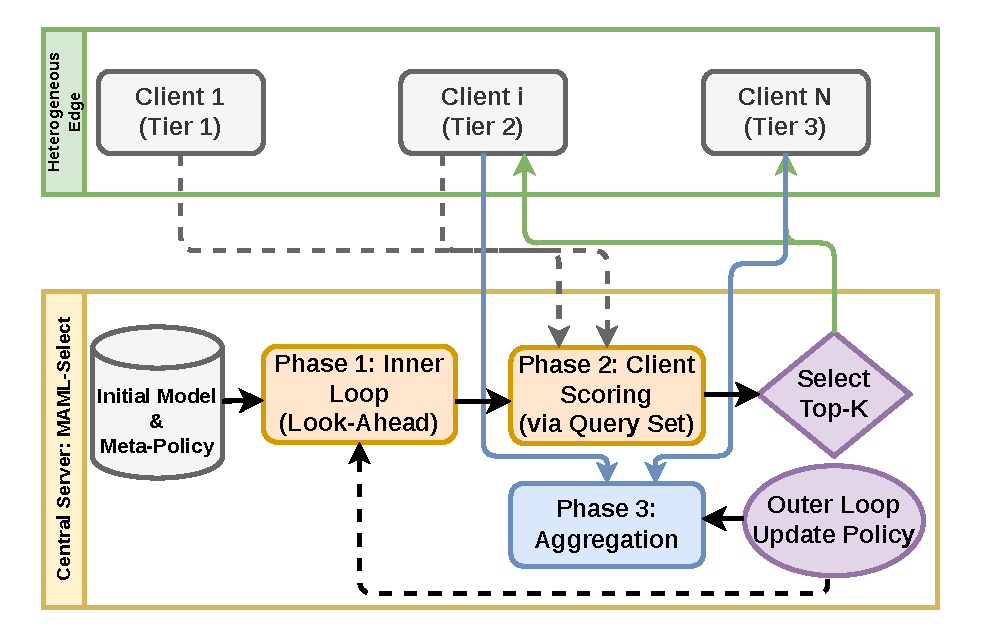
\includegraphics[width=0.82\columnwidth, trim={0.25cm 0.25cm 0.25cm 0.25cm},clip]{MAML.pdf}
\vspace{-2mm}
\caption{\revision{System model and MAML-Select workflow. A central server observes client states, selects $K$ clients from the available pool, aggregates their local updates, and uses returned local-loss and system feedback for support-set adaptation, candidate scoring, and query-set meta-update.}}
\vspace{-2mm}
\label{fig:model_diagram}
\end{figure}

\begin{algorithm}[!t]
	\vspace{-1mm}
	\caption{MAML-Select Algorithm}
	\label{alg:maml_select}
	\begin{algorithmic}[1]
		\scriptsize
		\State \textbf{Initialize:} Global model $\theta_0$; meta-policy parameters $\phi$; inner LR $\beta$; outer LR $\eta$; trade-off $\lambda$.
		\For{round $t = 1, \ldots, T$}
		\State Server broadcasts global model $\theta_t$ to all clients.
		\State Collect state vectors $\bm{s}_{i,t}$ from available clients.
		\If{$t > 1$}
		\State \texttt{// Phase 1: Inner Loop Adaptation}
		\State Construct $\mathcal{D}_{sup}$ from round $t-1$ results.
			\State \revision{Compute fast weights $\phi'_t$ using Eq.~\ref{eq:inner_loop}.}
		\Else
		\State $\phi'_t \leftarrow \phi_t$ \quad \texttt{// No adaptation for the first round}
		\EndIf
		\State \texttt{// Phase 2: Client Selection}
			\State \revision{Score clients: $\text{score}_i = h_{\phi'_t}(\bm{s}_{i,t})$ for all $i \in \mathcal{A}_t$.}
			\State \revision{Select lowest-cost clients: $\mathcal{S}_t \leftarrow \operatorname{Top-}K(-\text{scores})$.}
			\State \texttt{// FL Training Round}
				\State \revision{Receive local updates $\{\Delta\theta_{i,t}\}_{i \in \mathcal{S}_t}$, local losses, and system metrics.}
			\State \revision{Aggregate: $\theta_{t+1} \leftarrow \theta_t + \sum_{i \in \mathcal{S}_t} \frac{n_i}{\sum_{j \in \mathcal{S}_t}n_j}\Delta\theta_{i,t}$.}
			\State \texttt{// Phase 3: Outer Loop Meta-Update}
			\State Compute costs $c_{i,t}$ using Eq.~\ref{eq:cost} for $i \in \revision{\mathcal{S}_t}$.
			\State Construct $\mathcal{D}_{query}(t) = \{(\bm{s}_{i,t}, c_{i,t}) \mid i \in \revision{\mathcal{S}_t}\}$.
				\State \revision{Meta-update: $\phi_{t+1} \leftarrow \phi_t - \eta \nabla_{\phi'_t} \mathcal{L}_{query}(h_{\phi'_t};\mathcal{D}_{query}(t))$.}
		\EndFor
	\end{algorithmic}
\end{algorithm}

\revision{MAML-Select differs from fixed-rule selectors because its ranking policy is adapted before each decision. It also differs from RL selectors because the update is an explicit gradient step on recent support feedback. The method is designed for rapidly changing client utility.}

\subsubsection{Computational Complexity}
\revision{The meta-policy $h_\phi$ is a lightweight MLP with 4,673 parameters. Scoring $N$ available clients costs $\mathcal{O}(N|\phi|)$. One support-set adaptation and one query-set meta-update over a cohort of size $K$ cost $\mathcal{O}(K|\phi|)$. The total server-side policy cost per round is therefore $\mathcal{O}((N+K)|\phi|)$, excluding local model training. A supplementary scaling probe over $N=\{20,40,80,100\}$ clients confirms that the selector overhead remains at millisecond scale and is negligible relative to local training.}

% =====================================================================
% V. EVALUATION AND RESULTS
% =====================================================================
\section{Evaluation and Results}

\revision{We evaluate on three benchmarks: Fashion-MNIST using LightCNN-9~\cite{wu2018light} (lightweight IoT task), CIFAR-10 using ResNet18~\cite{he2016deep} (complex vision task), and CIFAR-100 using ResNet18 (100-class fine-grained task).} $N = 100$ clients are simulated with non-IID data partition (Dirichlet $\alpha = 0.5$), selecting $K = 10$ clients per round for $T = 200$ rounds (\revision{$150$ rounds for CIFAR-100}) with $E = 5$ local epochs and batch size 32. \revision{All results are reported as the mean over three random seeds ($42, 123, 2026$) wherever completed runs are available; standard deviations are shown when at least two seeds are available.} \revision{Local models use PyTorch default initialization and SGD with learning rate $0.01$, momentum $0.9$, weight decay $10^{-4}$, and a constant scheduler. The meta-policy uses one inner step with $\beta=0.01$ and Adam for the outer update with $\eta=0.001$; the selector seed is fixed to 2026.} \revision{Compute rates follow three device tiers inspired by mobile benchmarking studies~\cite{ignatov2018ai}: Tier~1 (20\%, $1.0\times$), Tier~2 (50\%, $2.0\times$), and Tier~3 (30\%, $4.0\times$).} The target latency deadline $T_{target}$ is set to the average round latency of Tier~2 clients, and the trade-off parameter $\lambda = 0.5$. \revision{Baselines include FedAvg (random selection), FedCS (system-aware deadline-constrained), Oort (utility-based with importance sampling), TiFL (tier-based), FedCor (correlation-based via Gaussian Processes), FedGCS (generative selection), and CriticalFL (critical-period cohort scaling).}

\subsection{\revision{Accuracy and Resource Cost}}
\revision{We estimate the client-training computation per round as}
\begin{equation}
	\text{TFLOPs}_{total} = \sum_{t=1}^{T} \sum_{i \in \mathcal{S}_t} E \cdot n_i \cdot C_{model} \times 10^{-12},
	\label{eq:tflops}
\end{equation}
\revision{where $C_{model}$ is the per-sample cost; for ResNet18 on CIFAR-10 a client round is approximately $4.13$ TFLOPs. Modelled energy and carbon scale this cost by per-tier device power and a declared grid intensity.}

\revision{Table~\ref{tab:main_summary} summarises all methods. MAML-Select attains accuracy on par with FedAvg and FedGCS on Fashion-MNIST ($90.1\%$ vs.\ $90.2\%$ and $90.7\%$) and CIFAR-100 ($58.2\%$ vs.\ $59.7\%$ and $58.7\%$), while clearly surpassing FedCS, Oort, TiFL, and FedCor. On CIFAR-10 it trades a small accuracy reduction ($75.6\%$ vs.\ FedAvg $79.4\%$) for substantially lower cost. On CIFAR-100, CriticalFL reaches only $48.8\%$ at the highest TFLOPs, energy, and communication of any method, whereas MAML-Select is both more accurate and far cheaper. The meta-update overhead ($\varepsilon \approx 0.001$ GFLOPs per round) is negligible relative to client training, and all selectors transmit identical communication volume.}

\begin{table*}[!t]
\centering
\caption{Benchmark summary across non-IID datasets. Accuracy, precision, recall, F1, and coverage are in percent; energy is in Wh and carbon is in gCO$_2$e. Standard deviations are shown where at least two completed seeds are available.}
\label{tab:main_summary}
\tiny
\setlength{\tabcolsep}{1.1pt}
\renewcommand{\arraystretch}{0.76}
\resizebox{0.88\textwidth}{!}{%
\begin{tabular}{@{}lrrrrrrrrr@{}}
\toprule
Method & Acc. & Prec. & Rec. & F1 & TFLOPs & Energy & Carbon & Jain & Cov. \\
\midrule
\multicolumn{10}{@{}l}{\textit{Fashion-MNIST}} \\
FedAvg & 90.22$\pm$0.58 & 90.55$\pm$0.20 & 90.22$\pm$0.58 & 90.22$\pm$0.51 & 140$\pm$1 & 5752$\pm$72 & 2732$\pm$34 & 0.95$\pm$0.00 & 100$\pm$0 \\
FedCS & 84.11$\pm$1.82 & 84.84$\pm$0.77 & 84.11$\pm$1.82 & 83.91$\pm$1.98 & 76$\pm$7 & 2772$\pm$211 & 1317$\pm$100 & 0.10$\pm$0.00 & 10$\pm$0 \\
Oort & 86.70$\pm$0.19 & 86.66$\pm$0.21 & 86.70$\pm$0.19 & 86.42$\pm$0.26 & 149$\pm$8 & 5963$\pm$456 & 2832$\pm$217 & 0.10$\pm$0.00 & 10$\pm$0 \\
TiFL & 86.73$\pm$0.34 & 86.62$\pm$0.26 & 86.73$\pm$0.34 & 86.51$\pm$0.34 & 147$\pm$6 & 6062$\pm$348 & 2879$\pm$165 & 0.11$\pm$0.00 & 12$\pm$0 \\
FedCor & 89.35$\pm$0.50 & 89.31$\pm$0.51 & 89.35$\pm$0.50 & 89.22$\pm$0.57 & 121$\pm$5 & 4845$\pm$204 & 2301$\pm$97 & 0.26$\pm$0.04 & 49$\pm$8 \\
CriticalFL & 89.83 & 89.98 & 89.83 & 89.81 & 405 & 16696 & 7931 & 0.99 & 100 \\
FedGCS & 90.65$\pm$0.29 & 90.73$\pm$0.16 & 90.65$\pm$0.29 & 90.63$\pm$0.26 & 136$\pm$4 & 5595$\pm$113 & 2658$\pm$54 & 0.95$\pm$0.02 & 100$\pm$0 \\
\textbf{MAML-Select} & 90.11$\pm$0.47 & 90.43$\pm$0.04 & 90.11$\pm$0.47 & 90.04$\pm$0.30 & 122$\pm$2 & 4809$\pm$79 & 2284$\pm$37 & 0.77$\pm$0.06 & 100$\pm$0 \\
\midrule
\multicolumn{10}{@{}l}{\textit{CIFAR-10}} \\
FedAvg & 79.43$\pm$1.84 & 80.01$\pm$1.28 & 79.43$\pm$1.84 & 79.36$\pm$1.78 & 8341$\pm$52 & 4798$\pm$24 & 2279$\pm$11 & 0.95$\pm$0.00 & 100$\pm$0 \\
FedCS & 50.45$\pm$2.57 & 50.88$\pm$2.60 & 50.45$\pm$2.57 & 49.87$\pm$2.33 & 4081$\pm$600 & 2073$\pm$262 & 985$\pm$125 & 0.10$\pm$0.00 & 10$\pm$0 \\
Oort & 60.19$\pm$5.18 & 60.84$\pm$4.97 & 60.19$\pm$5.18 & 59.69$\pm$4.61 & 8303$\pm$1923 & 4677$\pm$856 & 2222$\pm$406 & 0.10$\pm$0.00 & 10$\pm$0 \\
TiFL & 61.93$\pm$5.04 & 62.48$\pm$4.78 & 61.93$\pm$5.04 & 61.36$\pm$4.60 & 8200$\pm$2143 & 4800$\pm$1203 & 2280$\pm$572 & 0.11$\pm$0.00 & 12$\pm$0 \\
FedCor & 67.20$\pm$5.33 & 67.83$\pm$4.74 & 67.20$\pm$5.33 & 66.81$\pm$5.37 & 7748$\pm$695 & 4452$\pm$435 & 2115$\pm$206 & 0.20$\pm$0.02 & 31$\pm$5 \\
CriticalFL &  &  &  &  &  &  &  &  &  \\
FedGCS & 77.88$\pm$1.75 & 78.93$\pm$1.50 & 77.88$\pm$1.75 & 77.69$\pm$1.54 & 7656$\pm$278 & 4428$\pm$154 & 2103$\pm$73 & 0.90$\pm$0.03 & 100$\pm$0 \\
\textbf{MAML-Select} & 75.63$\pm$1.43 & 76.51$\pm$1.55 & 75.63$\pm$1.43 & 75.25$\pm$1.34 & 6549$\pm$118 & 3610$\pm$60 & 1715$\pm$29 & 0.61$\pm$0.01 & 100$\pm$0 \\
\midrule
\multicolumn{10}{@{}l}{\textit{CIFAR-100}} \\
FedAvg & 59.66$\pm$0.29 & 60.90$\pm$0.48 & 59.66$\pm$0.29 & 59.13$\pm$0.40 & 6331$\pm$6 & 3626$\pm$18 & 1722$\pm$9 & 0.94$\pm$0.00 & 100$\pm$0 \\
FedCS & 27.52$\pm$0.29 & 27.93$\pm$0.10 & 27.52$\pm$0.29 & 26.39$\pm$0.09 & 5334$\pm$23 & 2659$\pm$12 & 1263$\pm$6 & 0.10$\pm$0.00 & 10$\pm$0 \\
Oort & 29.41$\pm$1.73 & 29.82$\pm$1.77 & 29.41$\pm$1.73 & 28.13$\pm$1.73 & 5955$\pm$189 & 3421$\pm$181 & 1625$\pm$86 & 0.10$\pm$0.00 & 10$\pm$0 \\
TiFL & 32.12 & 33.07 & 32.12 & 31.02 & 5986 & 3499 & 1662 & 0.11 & 12 \\
FedCor & 34.18 & 33.89 & 34.18 & 32.93 & 6428 & 3668 & 1742 & 0.12 & 14 \\
CriticalFL & 48.84$\pm$1.58 & 60.56$\pm$1.89 & 48.84$\pm$1.58 & 48.07$\pm$2.32 & 9469$\pm$392 & 5438$\pm$214 & 2583$\pm$102 & 0.97$\pm$0.00 & 100$\pm$0 \\
FedGCS & 58.66$\pm$0.11 & 60.24$\pm$0.03 & 58.66$\pm$0.11 & 58.08$\pm$0.20 & 6140$\pm$24 & 3526$\pm$4 & 1675$\pm$2 & 0.82$\pm$0.02 & 100$\pm$0 \\
\textbf{MAML-Select} & 58.15$\pm$0.51 & 59.87$\pm$0.55 & 58.15$\pm$0.51 & 57.66$\pm$0.33 & 6224$\pm$20 & 3457$\pm$6 & 1642$\pm$3 & 0.78$\pm$0.03 & 100$\pm$0 \\
\bottomrule
\end{tabular}%
}
\end{table*}

\revision{Fig.~\ref{fig:convergence} summarises the CIFAR-100 round-wise behaviour. MAML-Select remains close to FedAvg and FedGCS on accuracy, precision, and loss while staying in the efficient carbon cluster. CriticalFL is costlier without an accuracy advantage in this setting.}

\begin{figure}[H]
\centering

\includegraphics[width=\columnwidth]{fig_convergence.pdf}
\caption{\revision{CIFAR-100 convergence over 150 rounds. The panels report accuracy, precision, cumulative modelled carbon, and test loss.}}
\label{fig:convergence}
\end{figure}

\revision{Fig.~\ref{fig:tradeoff} shows the efficiency--accuracy trade-off relative to FedAvg. Points to the left of $x=1$ use less cumulative training compute; points above $y=0$ improve accuracy. MAML-Select is consistently in the lower-compute region. Relative to FedAvg over shared seeds, it lowers cumulative TFLOPs by $12.8\%$/$21.5\%$/$1.7\%$ and modelled energy and carbon by $16.4\%$/$24.7\%$/$4.7\%$ on Fashion-MNIST/CIFAR-10/CIFAR-100. The corresponding accuracy changes are $-0.1$/$-3.8$/$-1.5$ percentage points. Thus the main empirical gain is resource efficiency with competitive, not universally superior, accuracy. This is the desired operating region for resource-constrained FL: the selector avoids the high-cost cohorts used by CriticalFL while retaining the data coverage needed for stable learning.}

\begin{figure}[H]
\centering

\includegraphics[width=0.78\columnwidth]{fig_tradeoff.pdf}
\caption{\revision{Efficiency--accuracy trade-off relative to FedAvg. $x<1$ indicates lower cumulative training compute, while $y$ reports accuracy change in percentage points.}}
\label{fig:tradeoff}
\end{figure}

\revision{MAML-Select reaches $100\%$ client coverage on every dataset. Its Jain index ($0.61$--$0.78$) is below FedAvg and FedGCS, so we do not claim improved fairness; the coverage result instead shows that the policy does not permanently exclude clients.}

\subsection{\revision{Sensitivity and Ablation}}
\revision{Fig.~\ref{fig:lambda_sensitivity} analyses $\lambda$ on Fashion-MNIST using four normalized curves: accuracy, compute, energy, and fairness. Final accuracy remains stable across $\lambda \in \{0.1, 0.5, 1, 5\}$, with about a $1.0$ percentage-point spread, while compute and energy decrease as the latency/resource term receives more weight. Fairness decreases more sharply for very large $\lambda$, indicating a stronger efficiency--fairness trade-off. We therefore use $\lambda=0.5$ as a balanced operating point: it keeps accuracy close to the best observed value while reducing computation relative to $\lambda=0.1$.}

\begin{figure}[H]
\centering

\includegraphics[width=0.76\columnwidth]{fig_lambda_sensitivity_multimetric.pdf}
\caption{\revision{$\lambda$ sensitivity on Fashion-MNIST. Curves are normalized to the value at $\lambda=0.1$ and report accuracy, compute, energy, and fairness.}}
\label{fig:lambda_sensitivity}
\end{figure}

\revision{Fig.~\ref{fig:feature_ablation} and Table~\ref{tab:ablation} show the state-feature ablation. Removing a single feature changes Fashion-MNIST accuracy by less than about $0.35$ percentage points. The largest negative shifts occur when battery and loss information are removed, showing that the policy benefits from both system and statistical feedback. Removing frequency or staleness can slightly increase accuracy but lowers fairness/coverage behaviour, so these features remain important for stable participation.}

\begin{figure}[H]
\centering

\includegraphics[width=0.78\columnwidth]{fig_feature_ablation_trimmed.pdf}
\caption{\revision{State-feature ablation on Fashion-MNIST. Each bar reports the accuracy change relative to the full six-feature state vector.}}
\label{fig:feature_ablation}
\end{figure}

\begin{table}[!t]
\vspace{-8mm}
\centering
\caption{State-feature ablation on Fashion-MNIST ($n=3$). Each row removes one feature from the
six-dimensional state vector; the full vector is the reference.}
\label{tab:ablation}
\scriptsize
\setlength{\tabcolsep}{3.4pt}
\renewcommand{\arraystretch}{0.92}
\begin{tabular*}{\columnwidth}{@{\extracolsep{\fill}}lrrr@{}}
\toprule
Variant & Acc.\ (\%) & TFLOPs & Jain \\
\midrule
\textbf{Full state vector} & 90.23\,$\pm$\,0.55 & 122 & 0.78 \\
w/o loss & 90.16\,$\pm$\,0.66 & 123 & 0.79 \\
w/o gradient norm & 90.30\,$\pm$\,0.24 & 122 & 0.78 \\
w/o latency & 90.14\,$\pm$\,0.14 & 119 & 0.70 \\
w/o battery & 89.90\,$\pm$\,0.44 & 122 & 0.79 \\
w/o frequency & 90.47\,$\pm$\,0.13 & 115 & 0.65 \\
w/o staleness & 90.37\,$\pm$\,0.19 & 123 & 0.78 \\
\bottomrule
\end{tabular*}
\vspace{-2mm}
\end{table}


% =====================================================================
% VI. CONCLUSION
% =====================================================================
\FloatBarrier
\section{Conclusion and Future Work}
\revision{We introduced MAML-Select, an online adaptive client-selection framework for heterogeneous FL. It learns a lightweight ranking policy and adapts it from recent feedback before each selection decision. Across Fashion-MNIST, CIFAR-10, and CIFAR-100, MAML-Select delivers competitive accuracy while lowering cumulative computation, modelled energy, and carbon. The $\lambda$-sensitivity and feature-ablation studies validate the design; future work will add hardware-level energy measurement and larger-scale benchmarks.}

% =====================================================================
% REFERENCES
% =====================================================================
\vspace{-1mm}
\bibliographystyle{IEEEtran}
\bibliography{References_letter}

\end{document}
